%=== CHAPTER FOUR ===
%% The coupled MHE-NMPC architecture, the continuous payload interface, and the
%% eventless grasp/release lifecycle.  Rewritten 2026-09-18 against the deployed
%% implementation.

\chapter{The Eventless MHE--NMPC Framework}
\label{ch:framework}
\begin{spacing}{1.5}
\setlength{\parskip}{0.22in}

Chapter~\ref{ch:model} established \emph{what} is estimated and why. This
chapter states \emph{how}: the numerical form of the two optimal control
problems, the interface that carries the estimate from one to the other, and the
logic that decides when the controller may believe that its payload has gone.

The organising principle of the chapter is stated once here and applied
throughout. \emph{No attach or release notification is evidence.} The controller
issues the gripper command itself, and still does not use it to update its model.
The only thing that clears a payload from the model is persistent estimator
evidence. Section~\ref{sec:frame:why-eventless} argues why a system that
possesses the command should nevertheless refuse to use it; the remainder of the
chapter builds the machinery that makes the refusal affordable.

\section{Closed-Loop Architecture}\label{sec:frame:arch}

Figure~\ref{fig:architecture} shows the information flow. Three layers are
involved: the physics and flight stack (Gazebo, PX4 software-in-the-loop, and a
magnetic detachable-joint gripper that produces genuine inertia and
centre-of-mass changes); the inner rate-control loop on the autopilot; and a ROS
outer loop containing the estimator and the predictive controller.

\begin{figure}[ht]
\centering
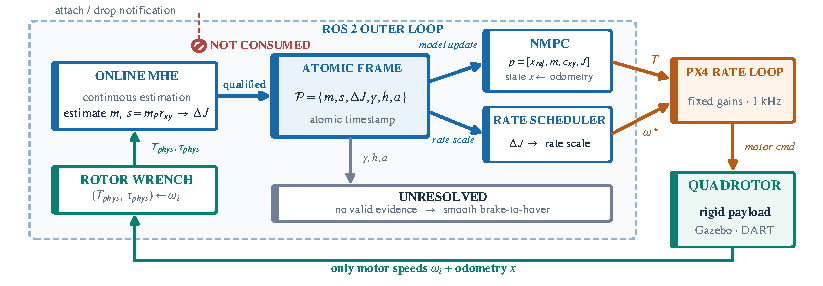
\includegraphics[width=0.98\textwidth]{Figures/fig1_architecture.pdf}
\caption{System architecture and information flow. The complete pipeline consumes
only rotor speeds and odometry. One atomic, health-gated $m/\svec/J$ frame drives
both the NMPC model and the continuous body-rate command scheduling. No
attach or release notification enters this path.}
\label{fig:architecture}
\end{figure}

Two properties of this diagram carry the argument of the dissertation.

First, \textbf{the only inputs are odometry and rotor speeds.} The estimator does
not read the controller's intended thrust or torque
(Section~\ref{sec:model:phys}), does not read the gripper's attach or release
record, and does not read the simulator's joint state. The payload truth
available in simulation is used exclusively for offline scoring.

Second, \textbf{there is exactly one interface.} The estimator publishes a single
atomic frame (Section~\ref{sec:frame:interface}) containing mass, first moment,
the derived geometry, a confidence scalar and a health flag. Both consumers ---
the NMPC model parameters and the inner-loop command scaling --- read that one
frame. An earlier design in which mass, geometry and inertia travelled on
separate topics, each with its own latency and validity, made it possible for the
controller to hold a mutually inconsistent parameter set; the atomic frame makes
that class of fault unrepresentable.

The two optimisers run at different rates and do not share a solve clock. The
estimator solves at \SI{10}{\hertz} over a \SI{2}{\second} window; the controller
solves at \SI{20}{\hertz} over a \SI{1}{\second} preview; setpoints are published
at \SI{50}{\hertz} by interpolating along the most recent predicted trajectory.

\section{Moving Horizon Estimator}\label{sec:frame:mhe}

\subsection{The optimisation}\label{sec:frame:mheocp}

With the augmented state \eqref{eq:xaug} of Chapter~\ref{ch:model}, the estimator
solves, at each \SI{10}{\hertz} tick,
\begin{align}
\min_{x_{0:N},\, w_{0:N-1}} \quad
& \bigl\| x_0 - \bar{x}_0 \bigr\|^2_{W_0}
+ \sum_{j=0}^{N-1} \beta_j \Bigl( \bigl\| y_j - C x_j \bigr\|^2_{W_y}
+ \bigl\| w_j \bigr\|^2_{W_w} \Bigr) \nonumber \\
\mathrm{s.t.} \quad
& x_{j+1} = F_{\mathrm{M}}\bigl(x_j,\, u^{\mathrm{phys}}_j\bigr) + G\,w_j, \nonumber \\
& \underline{m} \le \mT \le \overline{m}, \qquad
  |s_x|,\,|s_y| \le \overline{s},
\label{eq:mhe}
\end{align}
where $y_j$ is the odometry measurement, $C$ selects the thirteen vehicle states
from the sixteen-dimensional augmented state, $F_{\mathrm{M}}$ is one explicit
fourth-order Runge--Kutta step of the dynamics of Chapter~\ref{ch:model} driven
by the reconstructed wrench $u^{\mathrm{phys}}$ of \eqref{eq:phys}, and
\begin{equation}
G = \begin{bmatrix} I_{13} \\ 0_{3\times13}\end{bmatrix}
\label{eq:Gmat}
\end{equation}
confines the process noise to the physical states, leaving $\mT$ and $\svec$
noise-free within the window.

The horizon is $N=20$ stages at $\Delta t=\SI{0.1}{\second}$. The choice is a
compromise that the experiments of Chapter~\ref{ch:evaluation} revisit: a longer
window averages more measurement noise, but the constraint that makes the payload
states identifiable --- that they are \emph{constant} over the window --- becomes
less defensible the longer the arc of trajectory the window spans. On a
\SI{4}{\meter\per\second} figure-eight a ten-stage window recovered the mass
$3.7\times$ more accurately than a twenty-stage one, while a forty-stage window
sat on the lower bound for the entire flight.

\subsection{Weights}\label{sec:frame:weights}

All three weight matrices follow Bryson's rule: each diagonal entry is the
inverse square of a representative magnitude for the corresponding residual, so
that every channel contributes a cost of order unity at its own natural scale and
the Gauss--Newton Hessian is not curvature-imbalanced across directions.

The measurement weight uses representative state-estimation standard deviations,
\begin{equation}
W_y = \mathrm{diag}\Bigl(\sigma_p^{-2}I_3,\ \sigma_v^{-2}I_3,\ \sigma_q^{-2}I_4,\ \sigma_\omega^{-2}I_3\Bigr),
\label{eq:Wy}
\end{equation}
with $\sigma_p=\SI{0.02}{\meter}$, $\sigma_v=\SI{0.05}{\meter\per\second}$,
$\sigma_q=0.01$ (about \SI{1.1}{\degree}) and
$\sigma_\omega=\SI{0.02}{\radian\per\second}$.

The process-noise weight is deliberately \emph{tighter} than the measurement
weight,
\begin{equation}
W_w = \mathrm{diag}\bigl(10^{4} I_6,\ 10^{5} I_4,\ 10^{3} I_3\bigr).
\label{eq:Ww}
\end{equation}
This is the central tuning decision of the estimator, and its rationale is worth
stating explicitly. The purpose of \eqref{eq:mhe} is not to smooth noisy
measurements; it is to force any persistent mismatch between the reconstructed
wrench and the observed motion to be explained by the two payload parameters
rather than absorbed into unstructured process noise. Trusting the dynamics ---
large $W_w$ --- is what makes that attribution happen. The angular block is one
decade looser than the translational block because the rotational equation
contains the gyroscopic product $\bm\omega\times\Jt\bm\omega$ and the inverse
inertia, and is numerically the more delicate of the two.

The arrival cost anchors the start of the window,
\begin{equation}
W_0 = \mathrm{diag}\bigl(10^{3} I_6,\ 10^{4} I_4,\ 10^{2} I_3,\ \sigma_{m,0}^{-2},\ \sigma_{s,0}^{-2}I_2\bigr),
\qquad
\sigma_{m,0} = \SI{3.16}{\kg},\ \ \sigma_{s,0}=\SI{0.1}{\kg\meter},
\label{eq:W0}
\end{equation}
with $\bar x_0$ taken from the previous window's solution shifted forward by one
stage. Two points about the payload entries. First, they are four to five orders
of magnitude softer than the physical-state entries: with
$\sigma_{m,0}=\SI{3.16}{\kg}$ against a vehicle that weighs \SI{2.06}{\kg}
empty, the mass anchor carries essentially no information, and that is
intentional --- it is what allows a payload step to be absorbed within roughly
one window rather than being dragged toward the previous answer. Second, they are
not set to zero. A zero entry removes positive definiteness of the Hessian in
that direction whenever a window happens to be poorly excited, and an earlier
experiment with genuinely uninformative payload channels produced 472 solver
failures from exactly that mechanism. A numerically small but non-zero anchor is
uninformative in the statistical sense while remaining well posed in the
numerical one.

The bounds in \eqref{eq:mhe} are physical rather than tuning knobs. The
composite mass is constrained to
$[\,0.95\,\mB,\ \SI{5.0}{\kg}\,]=[\SI{1.961}{\kg},\SI{5.0}{\kg}]$: the vehicle
cannot weigh less than its own airframe, and the \SI{5}{\percent} margin leaves
room for calibration error rather than pinning the estimate at the calibrated
value. That such a bound is a \emph{hard constraint on a decision variable} is a
concrete advantage of the moving-horizon formulation over a recursive filter,
which can be biased away from non-physical estimates but cannot be forbidden from
producing them. The first moment is bounded loosely,
$\overline{s}=\SI{1.5}{\kg\meter}$, purely to prevent the optimiser from
diverging; the physically meaningful admissibility limit on $\svec$ is applied
later, in the reference-formation logic of Section~\ref{sec:frame:momentref},
where it can reject a sample without distorting the optimisation.

\paragraph{The prior-free ablation.} The lower bound $0.95\,\mB$ and the arrival
mean are the two remaining places where the airframe mass could in principle
inform the mass channel. The implementation therefore retains a switch that
removes both: the bound drops to \SI{0.2}{\kg} --- a value chosen only to keep
$1/\mT$ away from its singularity and containing no airframe information --- and
$\sigma_{m,0}$ rises to \SI{1000}{\kg}. This configuration is an
\emph{ablation}, not the deployed default; the results of
Chapter~\ref{ch:evaluation} are reported under the default unless stated
otherwise. The seed of Section~\ref{sec:model:seed} is prior-free in both
configurations, because it is computed from measurements in either case.

\subsection{Stage weighting: what was tried and what is deployed}\label{sec:frame:beta}

The factors $\beta_j$ in \eqref{eq:mhe} exist because the constant-payload model
is valid on either side of a grasp or release but not across one. When the event
falls inside the current window, a fixed-weight estimator returns a compromise
between two physical regimes until the older regime leaves the horizon --- a
transient on the order of the window length.

Three treatments were implemented and compared.

\paragraph{Event-triggered de-weighting (retired).} The original scheme detected a
persistent step in $\Tphys$ and scaled every stage preceding it by $10^{-4}$,
leaving the arrival cost active so that the physical-state trajectory remained
available as a warm start. On the \SI{2}{\meter\per\second} condition this
schedule remained armed but never fired. At \SI{4}{\meter\per\second} it was
\emph{disabled}, because grasp and release transients are not the only events
that move the collective thrust: a trajectory-mode change produces a step of the
same amplitude, and the detector cannot distinguish them. All results reported in
Chapter~\ref{ch:evaluation} use $\beta_j\equiv1$. A parameterised generalisation
of the schedule was additionally optimised by cross-entropy search, and found no
measurable improvement over the hand-designed rule; that negative result is
substantive, and is discussed in Section~\ref{sec:eval:weightlearning}.

\paragraph{Exponential forgetting (available, off by default).} A continuous
alternative discounts each stage by its age,
\begin{equation}
\beta_j = \lambda^{\,N-1-j}, \qquad j=0 \text{ oldest},
\label{eq:forget}
\end{equation}
giving an effective memory of about $1/(1-\lambda)$ stages --- ten frames
(\SI{1.0}{\second}) at $\lambda=0.9$, five at $\lambda=0.8$. This is the smooth
version of shortening the horizon: it neither changes the problem dimension nor
introduces a new noise channel, and the arrival-cost block is explicitly excluded
from the discount, since that block anchors physical states rather than carrying
stale payload evidence. The deployed default is $\lambda=1$.

\paragraph{Parameter random walk (available, off by default).} The third option
admits process noise on the payload channels themselves, replacing
$\dot{\mT}=0$, $\dot{\svec}=\bm 0$ by a random walk with tuned intensities
$\sigma_{\dot m}$ and $\sigma_{\dot s}$, as is standard in the learned-MHE
literature \cite{neuromhe}. It removes the need for any event logic, since the
parameters can then move within a window. It is off by default because the added
noise channels have natural scales two orders of magnitude apart from the
physical ones, and the resulting Hessian conditioning produced the 472 solver
failures noted above.

The deployed configuration therefore uses no event logic at all. This is a
deliberate simplification and it costs a transient of roughly one window after
each payload change; the lifecycle logic of Section~\ref{sec:frame:lifecycle} is
built to tolerate that transient rather than to shorten it.

\subsection{Re-anchoring and over-range rejection}\label{sec:frame:reanchor}

Two guards protect the estimator from its own failures.

\paragraph{Re-anchoring after repeated solver failure.} After five consecutive
failed solves the window is discarded and rebuilt: the physical states are reset
to the current measurement, the mass is re-seeded from \eqref{eq:winbal}, and
$\svec$ is reset to zero. The choice of zero is not neutral --- it asserts ``no
payload'' --- and it therefore has a consequence that the release logic must
respect: a first moment that is zero \emph{because the window was just rebuilt}
is not evidence of a release. Section~\ref{sec:frame:decision} states that rule
explicitly.

\paragraph{Physically inadmissible first moments.} The platform cannot realise a
first moment larger than
\begin{equation}
\lVert\svec\rVert_{\max} = \mP^{\mathrm{env}}\, r_{xy}^{\max}
= \SI{0.30}{\kg}\times\SI{0.13}{\meter} = \SI{0.039}{\kg\meter},
\label{eq:sadmissible}
\end{equation}
so a solved $\lVert\hat\svec\rVert$ above that bound is a statement about the
estimator, not about the payload. Such samples are excluded from the
reference-formation window of Section~\ref{sec:frame:momentref} and counted as an
estimator-quality diagnostic; if they persist while the vehicle is not
manoeuvring, the window is re-anchored. They are \emph{not} removed from the
published frame, which is a limitation recorded in Chapter~\ref{ch:evaluation}:
an out-of-envelope $\hat\svec$ still reaches the controller's $\cvec$ through the
filter and slew limiter.

\section{The Continuous Payload Interface}\label{sec:frame:interface}

\subsection{One atomic frame}\label{sec:frame:frame}

After each solve the estimator publishes
\begin{equation}
\mathcal{P} = \Bigl\{\, \mT,\; s_x, s_y,\; c_x, c_y,\;
\dJ_{xx},\dJ_{yy},\dJ_{zz},\; J_{xx},J_{yy},J_{zz},\; \gamma,\; h,\; a \,\Bigr\},
\label{eq:frame}
\end{equation}
in which the geometry entries are computed from $(\mT,\svec)$ by
\eqref{eq:c_from_s} and \eqref{eq:Jdeployed}, $\gamma\in[0,1]$ is the no-payload
confidence of Section~\ref{sec:frame:gamma}, $h$ is a health bit and $a$ is the
age of the most recent successful solution.

Health is a conjunction: the latest solve must have succeeded, and the odometry,
rotor-speed and known-input streams must all be fresher than
\SI{0.30}{\second}. The consumer applies one further test of its own, on the
receive age of the frame itself (\SI{0.35}{\second}), because a frame can be
healthy at the moment it is produced and stale by the time it is used.

The asymmetry in how an unhealthy frame is treated is deliberate and is the
safety property of the interface: \emph{an unhealthy or stale frame freezes the
last accepted model and resets the confidence persistence timer}. A degraded
estimate can therefore delay a release confirmation, but it can never cause one.

\subsection{Filtering and slew limiting}\label{sec:frame:filter}

A valid frame is not consumed directly. Each channel passes a first-order
low-pass filter and a separate rate limiter before it reaches the solver:
\begin{equation}
\alpha = 1 - e^{-\Delta t/\tau},
\qquad
\hat\theta \;\leftarrow\; \hat\theta + \alpha\bigl(\theta^{\mathrm{tgt}} - \hat\theta\bigr),
\qquad
\hat\theta \;\leftarrow\; \hat\theta + \mathrm{clip}\bigl(\cdot,\ \pm \dot\theta_{\max}\Delta t\bigr),
\label{eq:lpfslew}
\end{equation}
with $\tau=\SI{0.20}{\second}$ on the controller side
($\SI{0.25}{\second}$ on the estimator's own output stage) and rate limits
$\SI{0.60}{\kg\per\second}$ for the mass, $\SI{0.080}{\kg\meter\per\second}$ for
the first moment and $\SI{0.080}{\kg\meter\squared\per\second}$ for the inertia
increment.

The reason for a limiter in addition to a filter is that the two protect against
different things. The filter attenuates noise; the limiter bounds how fast the
\emph{model} underneath a receding-horizon optimisation may change. A parameter
step between consecutive solves invalidates the warm start, and an optimiser that
must re-converge from scratch at \SI{20}{\hertz} is an optimiser that
occasionally does not converge in time. The limiter converts any step ---
including a genuine one at grasp --- into a ramp the solver can track.

\section{The Eventless Grasp--Release Lifecycle}\label{sec:frame:lifecycle}

\subsection{Why refuse the command}\label{sec:frame:why-eventless}

The controller in this work issues the gripper-release command itself. It would
be trivial to clear the payload model at that instant, and every command-triggered
implementation does so. The reason not to is that a release command is a
\emph{request}, and the model must describe the \emph{vehicle}.

The two diverge in practice. A gripper can be slow to open, can jam, can release
only part of a multi-item load, or can release nothing at all; conversely, a load
can be torn off, can slip, or can be released by an agent whose notification
never arrives. In each case a command-triggered controller flies a loaded vehicle
with an empty model, or an empty vehicle with a loaded one. The failure is silent,
because nothing in the control loop contradicts it.

The eventless alternative accepts a cost --- confirmation is delayed by the time
the estimator needs to accumulate evidence --- in exchange for a model that is
never wrong for a reason the vehicle cannot detect.
Chapter~\ref{ch:evaluation} measures both sides of that trade.

\subsection{Two state machines}\label{sec:frame:fsm}

The lifecycle is split between the two nodes, as shown in
Figure~\ref{fig:fsm}. The estimator owns payload \emph{presence} and may
\emph{declare} a release. The controller owns the payload \emph{model} and clears
it only on \emph{confirmation}. Declaration is neither necessary nor sufficient
for confirmation; the separation exists so that a single detector cannot, by
itself, empty the controller's model.

\begin{figure}[ht]
\centering
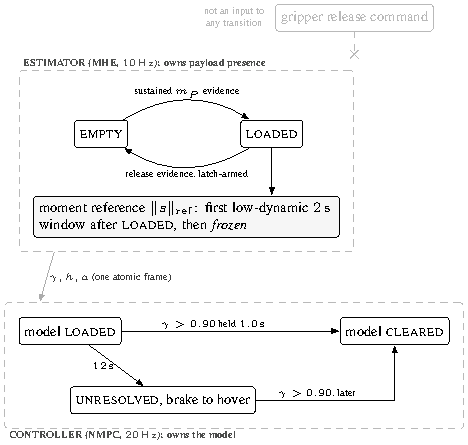
\includegraphics[width=0.92\textwidth]{Figures/fig_lifecycle_fsm.pdf}
\caption{The payload lifecycle as two state machines. The estimator owns payload
presence and may declare release from the evidence of
\eqref{eq:release-evidence}; the controller owns the model and clears it only on
confirmation, $\gamma>0.90$ held for \SI{1.0}{\second}. The gripper release
command enters neither machine. \textsc{unresolved} is a hold, not a clearing:
the model stays loaded while the vehicle brakes to hover and keeps waiting for
evidence.}
\label{fig:fsm}
\end{figure}

Presence is a hysteretic \textsc{empty}$\leftrightarrow$\textsc{loaded} machine
driven by sustained payload-mass evidence, with a directional thrust residual as
a fast path into \textsc{loaded}. A separate latch records that the present
flight reliably entered \textsc{loaded} at some point. That latch does two jobs:
it prevents an empty-flight confidence value from consuming the later release
confirmation, and it prevents a transient mass dip during the figure-eight from
disarming the true release path.

\subsection{No-payload confidence}\label{sec:frame:gamma}

Every lifecycle decision is a function of the published frame \eqref{eq:frame}
alone. The confidence scalar $\gamma$ fuses three ``empty'' indications.

Let $\sigma(v;a,b)$ be the smooth indicator that is $1$ for $|v|\le a$, $0$ for
$|v|\ge b$, and in between
\begin{equation}
\sigma(v;a,b) = 1 - \bigl(3\chi^2 - 2\chi^3\bigr),
\qquad \chi = \frac{|v|-a}{b-a},
\label{eq:smoothstep}
\end{equation}
which is the standard cubic smooth-step: continuous with continuous first
derivative at both ends, so $\gamma$ cannot jump when a channel crosses a
threshold. Then
\begin{equation}
\gamma \;=\; \sigma\bigl(\mP;\,0.015,\,0.060\bigr)\;\cdot\;
             \sigma\bigl(\lVert\svec\rVert;\,0.0015,\,0.0060\bigr)\;\cdot\;
             \sigma\bigl(\dJ_{xy};\,0.0020,\,0.0100\bigr),
\label{eq:gamma}
\end{equation}
with thresholds in \si{\kg}, \si{\kg\meter} and \si{\kg\meter\squared}, and
$\dJ_{xy}=\max(|\dJ_{xx}|,|\dJ_{yy}|)$.

The choice of a \emph{product} rather than a sum or a vote is deliberate: any
single payload indication vetoes \textsc{empty}. In particular a non-zero first
moment keeps $\gamma$ low even when the scalar mass estimate happens to be
sitting on its lower bound --- which, as Section~\ref{sec:model:whyS} showed, is
exactly the state the predecessor design entered after a release. The product
turns that failure mode into a refusal to confirm rather than a false
confirmation.

It is worth being precise that \eqref{eq:gamma} is a \emph{state-quality} metric
for a payload that has already gone, not a transition detector. The moment factor
carries an absolute threshold, and a state transition must not depend on the
estimator's noise floor happening to lie below an absolute number. The release
detector of Section~\ref{sec:frame:decision} therefore uses the individual
indications, not their product.

\subsection{The loaded moment reference}\label{sec:frame:momentref}

The release detector is built on a \emph{ratio},
\begin{equation}
\rho \;=\; \frac{\lVert\svec\rVert}{\sref},
\label{eq:rho}
\end{equation}
and the reason is empirical. Over five development flights the loaded and
released distributions of $\lVert\svec\rVert$ \emph{overlap}: the loaded minimum,
\SI{0.0039}{\kg\meter}, lies below the released maximum,
\SI{0.0049}{\kg\meter}. No absolute threshold separates them. The ratio does,
because it compares the vehicle against itself.

That requires a reference the estimator must form autonomously. A running maximum
is not acceptable --- it would absorb precisely the figure-eight estimation
errors the detector exists to reject, and \SIrange{7.6}{18.3}{\percent} of loaded
frames exceed the physical bound \eqref{eq:sadmissible} during the manoeuvre,
which would depress the denominator until $\rho$ crossed its threshold with the
payload still attached. The deployed procedure instead forms a reference once and
freezes it:

\begin{enumerate}
\item \textbf{Admissibility.} After the \textsc{loaded} declaration, a healthy
frame is admitted only if $\lVert\hat\svec\rVert\le\SI{0.039}{\kg\meter}$ by
\eqref{eq:sadmissible}. An out-of-envelope sample is discarded, not clipped:
clipping would still build the denominator from a sample known to be wrong.

\item \textbf{Low dynamics.} The vehicle must satisfy
$\lVert\bm\omega\rVert\le\SI{0.15}{\radian\per\second}$ and
$\lVert\bm v_{xy}\rVert\le\SI{0.20}{\meter\per\second}$. This is an
\emph{online} criterion, not ``wait $N$ seconds after grasp'': the latter would
only be correct for one particular mission script.

\item \textbf{Persistence.} Twenty consecutive admitted frames
(\SI{2}{\second}) must accumulate; any manoeuvre clears the buffer.

\item \textbf{Magnitude stability.} The window must satisfy
\begin{equation}
\frac{1.4826\cdot\mathrm{MAD}\bigl(\lVert\svec_j\rVert\bigr)}
     {\mathrm{median}\bigl(\lVert\svec_j\rVert\bigr)} \;\le\; 0.25,
\label{eq:madcv}
\end{equation}
where the factor $1.4826$ converts the median absolute deviation into a
consistent estimate of the standard deviation for Gaussian data. A robust
dispersion measure is used rather than the sample standard deviation because a
single outlying frame must not be able to veto an otherwise clean window.

\item \textbf{Direction consistency.} The window must further satisfy
\begin{equation}
\Bigl\lVert \frac{1}{20}\sum_{j} \frac{\svec_j}{\lVert\svec_j\rVert} \Bigr\rVert \;\ge\; 0.90 ,
\label{eq:dirmean}
\end{equation}
that is, the mean \emph{unit} first-moment vector must be close to unit length.
This catches the failure mode that \eqref{eq:madcv} cannot: a sequence whose
magnitude is perfectly steady while its direction rotates or flips sign frame to
frame, which is the signature of an ill-conditioned rotational channel rather
than of a real eccentric load.

\item \textbf{Robust statistic and freeze.} The reference is the
\SI{20}{\percent}-trimmed mean of the window magnitudes, and it is frozen for the
remainder of the flight.
\end{enumerate}

If no window qualifies before the vehicle enters the aggressive segment, $\rho$
never becomes available and the moment-gated path cannot fire. That is a genuine
miss mode, and it is the dominant one in the results of
Chapter~\ref{ch:evaluation}.

\subsection{Release evidence and the decision rule}\label{sec:frame:decision}

The detector organises its inputs into three \emph{independent} information
sources. The word is used strictly: an earlier version counted the mass channel
and the inertia channel as two votes, which was false robustness, since in the
continuous interface $\dJ=A(\mP)$ is a deterministic function of the mass and the
fixed $r_z$. They carry one piece of evidence, not two.

\begin{equation}
\begin{aligned}
\text{moment collapse}\quad&:\quad \rho < 0.30 \ \wedge\ \lVert\svec\rVert < \SI{0.008}{\kg\meter},\\
\text{quantity empty}\quad&:\quad \mP < \SI{0.030}{\kg},\\
\text{residual drop}\quad&:\quad \text{a signed thrust step, Section~\ref{sec:frame:resid}.}
\end{aligned}
\label{eq:release-evidence}
\end{equation}
The absolute bound in the first line is a sanity limit, not a discriminator ---
the distributions overlap, as noted above --- and it exists only to reject the
case in which an anomalously large reference peak makes $\rho$ spuriously small.

The decision rule is then
\begin{equation}
\text{release} \;\Longleftrightarrow\; \text{armed} \ \wedge\ \bigl[\, \text{slow path} \ \vee\ \text{fast path} \,\bigr],
\label{eq:releasedecision}
\end{equation}
in which
\begin{equation}
\begin{aligned}
\text{slow path}\;:\quad & \text{quantity empty} \ \wedge\ \text{moment collapse},
  \ \text{sustained } 5 \text{ frames},\\
\text{fast path}\;:\quad & \text{strong residual} \ \wedge\ \text{moment collapse},
  \ \text{sustained } 4 \text{ frames},
\end{aligned}
\label{eq:releasepaths}
\end{equation}
where \emph{armed} records that the present flight reliably entered
\textsc{loaded} at some earlier point.

\textbf{Moment evidence is mandatory in both paths}, and the reason is a recorded
failure. An earlier rule admitted a third path --- residual together with
quantity-empty, without moment evidence --- and it released prematurely in 3 of 9
randomised flights, the earliest \SI{51.1}{\second} before the release command.
Its design assumption, that ``quantity empty is false while the payload is
attached'', is simply untrue at \SI{4}{\meter\per\second}: the mass estimate sits
on its lower bound for whole stretches of a figure-eight, so $\mP$ is
persistently below \SI{0.03}{\kg} for a median of \SI{14}{\second} and as long as
\SI{48}{\second} in loaded flight. Neither amplitude nor persistence separates
that from a real release. The plain residual vote is likewise false-positive
during manoeuvre. The discarded path was therefore two unreliable channels
conjoined, with nothing able to veto them. The moment channel is the one that
measured cleanly: across those same flights the loaded $\rho$ bottomed at
$0.789$ against a threshold of $0.30$, a factor of $2.6$ of margin, with zero
false positives.

The cost of making moment evidence mandatory is accepted explicitly: \emph{a
release whose $\rho$ never collapses is not detected here.} That is a miss, and
it is handled by the \textsc{unresolved} path of
Section~\ref{sec:frame:unresolved} --- never by releasing on weaker evidence.

Two further rules close known loopholes. First, moment evidence must come from a
fresh, successful solve: the re-anchoring of Section~\ref{sec:frame:reanchor}
initialises $\svec$ to zero, and that zero is not counted as a collapse. Second,
the online and offline evaluations call the same pure decision function, so a
replay of a recorded flight exercises exactly the deployed logic rather than a
re-implementation of it.

\subsection{The release-residual vote}\label{sec:frame:resid}

The residual channel compares two adjacent half-windows of the reconstructed
collective thrust,
\begin{equation}
\Delta T_k \;=\; \overline{T}_{\mathrm{post}} - \overline{T}_{\mathrm{pre}}
\;=\; \frac{1}{h}\sum_{i=k-h+1}^{k} T^{\mathrm{phys}}_{i}
\;-\; \frac{1}{h}\sum_{i=k-2h+1}^{k-h} T^{\mathrm{phys}}_{i} ,
\qquad h=3 ,
\label{eq:deltaT}
\end{equation}
that is, two \SI{0.3}{\second} means at \SI{10}{\hertz}. A release makes
$\Delta T$ negative, because the vehicle no longer supports the load.

Amplitude alone is not enough: a recorded figure-eight transient reached
\SI{-1.69}{\newton}, which is larger in magnitude than the \SI{-1.47}{\newton}
weight of the smallest payload tested. The vote therefore combines a floor with a
robust significance test against the recent history of $\Delta T$ itself,
\begin{equation}
\hat\sigma_{\Delta T} = \max\Bigl(1.4826\cdot\mathrm{MAD}\bigl(\{\Delta T_i\}_{i<k}\bigr),\ \SI{0.05}{\newton}\Bigr),
\qquad
z_k = \frac{-\Delta T_k}{\hat\sigma_{\Delta T}} ,
\label{eq:deltaTz}
\end{equation}
where the history deliberately excludes the current frame, since a step included
in its own dispersion estimate inflates $\hat\sigma$ and hides itself. A vote is
cast when $\Delta T_k<\SI{-0.9}{\newton}$ persists for two frames, and a
\emph{strong} vote --- the one eligible to pair with a moment collapse in
\eqref{eq:releasedecision} --- when it persists for four.

Residual votes are \emph{edge} events and are given an explicit validity window
of \SI{3}{\second}. A vote that has expired is no longer evidence. This is a
small detail with a large consequence: without it, a single manoeuvre transient
early in a flight would remain available to be combined with an unrelated moment
collapse minutes later.

\subsection{Confirmation, \textsc{unresolved}, and braking to hover}\label{sec:frame:unresolved}

The controller clears its payload model through exactly one route:
\begin{equation}
\gamma > 0.90 \quad\text{held for}\quad \SI{1.0}{\second}
\quad\text{on healthy, fresh frames.}
\label{eq:confirm}
\end{equation}
An estimator declaration accelerates this but does not bypass it. On accepted
release evidence the estimator switches only the \emph{published target} of
$\svec$ to zero; the optimisation state is not overwritten. The output filter of
\eqref{eq:lpfslew} consequently produces a continuous decay rather than a
geometric step, and $\gamma$ rises smoothly through \eqref{eq:gamma}.
Confirmation can also occur with no declaration at all, driven by the estimator
converging on its own; the moment factor in \eqref{eq:gamma} still vetoes it
while $\lVert\svec\rVert$ is non-zero.

If no confirmation arrives within \SI{12}{\second} of the release command, the
controller enters \textsc{unresolved}. This state is the reason the eventless
design is deployable, and its semantics deserve emphasis: \textbf{a timeout is
not a release}. The model stays loaded. What changes is the vehicle's exposure:
it stops flying an aggressive trajectory it may no longer have the authority to
fly, and it gives the estimator a quiet operating point in which
Section~\ref{sec:frame:momentref}'s low-dynamic criterion can finally be met.

The braking manoeuvre is a finite-time reference rather than an instantaneous
switch to hover, because at \SI{4}{\meter\per\second} the latter would command a
step of several metres per second. Let $\bm p_0,\bm v_0$ be the state at the
declaration and $T_b=\SI{3}{\second}$. The stopping point is chosen as the
displacement of a constant deceleration from $\bm v_0$ to rest,
\begin{equation}
\bm p_1 = \bm p_0 + \tfrac{1}{2} T_b\, \bm v_0 ,
\label{eq:brakep1}
\end{equation}
and the reference between the two is the unique quintic satisfying
$\bm p(0)=\bm p_0$, $\dot{\bm p}(0)=\bm v_0$, $\ddot{\bm p}(0)=\bm 0$,
$\bm p(T_b)=\bm p_1$, $\dot{\bm p}(T_b)=\bm 0$, $\ddot{\bm p}(T_b)=\bm 0$:
\begin{equation}
\bm p(t) = \bm p_0 + \bm v_0 t + a_3 t^3 + a_4 t^4 + a_5 t^5,
\qquad
\begin{aligned}
a_3 &= \bigl(10\,\Delta\bm p - 6 T_b \bm v_0\bigr)/T_b^3,\\
a_4 &= \bigl(-15\,\Delta\bm p + 8 T_b \bm v_0\bigr)/T_b^4,\\
a_5 &= \bigl(6\,\Delta\bm p - 3 T_b \bm v_0\bigr)/T_b^5,
\end{aligned}
\label{eq:quintic}
\end{equation}
with $\Delta\bm p=\bm p_1-\bm p_0$. Zero acceleration at both ends means the
manoeuvre begins and ends without a jump in commanded thrust, which is what
keeps the transition from itself perturbing the estimator whose evidence is being
awaited. Attitude is blended over the same interval by the smooth-step of
\eqref{eq:smoothstep}.

\subsection{Threshold provenance}\label{sec:frame:thresholds}

Table~\ref{tab:thresholds} lists every lifecycle threshold and where its value
came from. All were fixed in code before the final campaign began and were not
retuned on it. Only the ratio threshold and the residual floor were selected
against data, and that data is from earlier flights that are disjoint from the
reported campaign; the remainder are engineering choices whose closed-loop
sensitivity has not been swept, and are reported as such.

\begin{table}[ht]
\centering
\caption{Lifecycle thresholds and their provenance. ``Earlier flights'' predate,
and are disjoint from, the reported campaign.}
\label{tab:thresholds}
\small
\begin{tabularx}{\textwidth}{@{}p{0.26\textwidth} p{0.20\textwidth} X@{}}
\toprule
\textbf{Threshold} & \textbf{Value} & \textbf{Provenance} \\
\midrule
moment-collapse ratio $\rho$ & $0.30$ &
leave-one-out cross-validation on 59 earlier flights; every fold selected
$0.30$, whereas $0.20$ succeeded in only 48 of 59 \\
residual floor / persistence & \SI{0.9}{\newton}; 2 or 4 frames &
below the \SI{1.47}{\newton} weight of the smallest payload; on a recorded
flight, figure-eight excursions past \SI{0.9}{\newton} lasted at most three
frames while the release step lasted four \\
slow-path persistence & 5 frames (\SI{0.5}{\second}) & engineering choice \\
mass-domain release & $\mP<\SI{0.030}{\kg}$, 20 frames &
between the loaded minimum (\SI{0.079}{\kg}) and the post-release maximum
(\SI{0.007}{\kg}) of earlier \SI{0.15}{\kg} flights \\
no-payload confidence & $0.90$ held \SI{1.0}{\second} & engineering choice \\
reference window & 20 frames; $\mathrm{CV}\le0.25$; direction $\ge0.90$ & engineering choice \\
\textsc{unresolved} timeout / brake & \SI{12}{\second} / \SI{3}{\second} & engineering choice \\
\bottomrule
\end{tabularx}
\end{table}

\section{Adaptive NMPC}\label{sec:frame:nmpc}

\subsection{Cost and weights}\label{sec:frame:nmpcweights}

The controller solves \eqref{eq:nmpc} with $N=20$ stages at
$\Delta t=\SI{0.05}{\second}$, preserving a \SI{1.0}{\second} preview while
running at \SI{20}{\hertz}. The residual vector is
\begin{equation}
\begin{aligned}
y_k = \bigl[\, &\bm e_p;\ \bm e_v;\ \bm e_{q,\mathrm{vec}};\ \bm e_\omega;\\
&u_k - u_{\mathrm{hover}}(p) \,\bigr] \in \mathbb{R}^{16},
\end{aligned}
\label{eq:nmpcresidual}
\end{equation}
where the attitude entry is the vector part of the relative quaternion
$\bm q_{\mathrm{ref}}^{*}\otimes\bm q$, which keeps the residual on the tangent
space of the rotation manifold instead of treating four quaternion components as
independent Euclidean coordinates.

Weights again follow Bryson's rule, $Q_{ii}=L_i^{-2}$, with tolerances
\begin{equation}
L_p=\SI{0.1}{\meter},\quad
L_v=\SI{0.3}{\meter\per\second},\quad
L_q=0.05,\quad
L_\omega=\SI{0.3}{\radian\per\second},
\label{eq:Lstate}
\end{equation}
and, on the inputs,
$L_T=\SI{2}{\newton}$, $L_{\tau,xy}=\SI{0.5}{\newton\meter}$,
$L_{\tau,z}=\SI{0.2}{\newton\meter}$; the torque scales are taken to be the
constraint bounds themselves, since the input cannot exceed them in any case. The
terminal weight rescales the stage blocks by $20$ (position), $1$ (velocity), $2$
(attitude) and $0.2$ (rate): the endpoint of the prediction is pulled tightly
onto the reference in position and attitude, while relaxing the terminal rate
demonstrably helps the solver.

This non-dimensionalisation is not cosmetic. Before it was applied, position and
torque weights differed by a factor of tens at their natural magnitudes, the
Gauss--Newton Hessian was correspondingly ill-conditioned across directions, and
the stationarity residual was observed to reach $6.26\times10^{5}$ --- a complete
numerical breakdown rather than a slow convergence.

\paragraph{Trajectory-scaled tolerances.} Two of the entries in \eqref{eq:Lstate}
are defined by the comment that accompanies them as trajectory-dependent
quantities: $L_v$ is a characteristic speed and $L_\omega$ a characteristic yaw
rate. Written as constants they are correct only for the low-speed reference they
were tuned on. An optional rescaling restores the intent,
\begin{equation}
L_v \leftarrow \max\bigl(L_v,\ r\,w\bigr),
\qquad
L_\omega \leftarrow \max\bigl(L_\omega,\ K_\psi\, w\bigr),
\qquad K_\psi = 3.17,
\label{eq:trajscale}
\end{equation}
taking the maximum so that the weights are only ever relaxed, never tightened.
The constant $K_\psi$ is the ratio of peak yaw rate to angular rate on the
figure-eight of Section~\ref{sec:frame:ref}, obtained numerically; it is worth
noting that evaluating the yaw rate at the intuitive location $a=\pi/4$ gives
$2.83$ and underestimates the peak by \SI{12}{\percent}, because the extremum
does not occur there. Applying \eqref{eq:trajscale} at the low-speed condition
reproduces $L_v$ exactly but relaxes $L_\omega$ by a factor of $3.2$, which
exposes a pre-existing mismatch rather than introducing one: the original value
was documented as matching a \emph{circular} trajectory, whose yaw rate is
constant at $w$, while the vehicle actually flies a figure-eight whose peak is
$3.17w$. The rescaling is off by default so that historical batches remain
reproducible.

\subsection{Solver}\label{sec:frame:solver}

Both optimal control problems are transcribed by direct multiple shooting with
explicit fourth-order Runge--Kutta integration, a Gauss--Newton Hessian
approximation, and partial-condensing HPIPM \cite{hpipm} as the quadratic
subproblem solver, generated and solved with acados \cite{acados}. Both use
\emph{full} sequential quadratic programming with merit-function backtracking
rather than the real-time-iteration scheme \cite{diehl2005rti}: RTI was observed
to diverge silently in this configuration, and a controller that reports success
while producing a diverging input is worse than one that takes an extra
millisecond. Generated C code is cached and reused until the model or problem
dimensions change.

\section{Inner-Loop Scheduling}\label{sec:frame:omegascale}

\subsection{From inertia ratio to a command scale}\label{sec:frame:scale}

Section~\ref{sec:model:gain} established that a five-fold inertia increase costs
the autopilot's rate loop most of its bandwidth, and that the outer loop cannot
recover it by being more accurate. The deployed response scales the body-rate
\emph{command} around the current measured rate,
\begin{equation}
\bm\omega_{\mathrm{cmd}}' \;=\; \bm\omega \;+\; \varsigma\,\bigl(\bm\omega_{\mathrm{cmd}} - \bm\omega\bigr),
\qquad \varsigma \ge 1,
\label{eq:omegascale}
\end{equation}
applied to the roll and pitch channels only, since $\dJ$ enters only $J_{xx}$ and
$J_{yy}$. Equation~\eqref{eq:omegascale} exaggerates the rate \emph{error} the
inner loop sees, which is equivalent to raising its proportional gain, without
modifying any autopilot parameter. Because it is a common scale on the roll/pitch
pair it preserves the direction of the rate-error vector.

The requested scale is the inertia ratio \eqref{eq:gain}, clipped at a cap of
$5.0$, evaluated from the live $\dJ$ of the payload frame. Three filters stand
between the request and its application, each addressing a distinct failure:

\begin{itemize}
\item a \textbf{dead band} of $0.08$ on the target, so that estimator noise
cannot move it, with explicit snapping to $1.0$ and to the cap so that hysteresis
cannot strand the empty-airframe steady state permanently above unity;
\item a \textbf{first-order filter} with $\tau=\SI{0.5}{\second}$, chosen far
slower than the inner loop (hundreds of hertz) and still fast enough to follow the
second-scale progressive load transfer during a grasp;
\item \textbf{asymmetric rate limits}, \SI{4.0}{\per\second} rising against
\SI{1.5}{\per\second} recovering, encoding the asymmetry of the consequences:
being late to add authority risks saturation, being late to remove it does not.
\end{itemize}

\subsection{Headroom limiting}\label{sec:frame:headroom}

Scaling a command that is already close to the rate limit accomplishes nothing
except saturation, at which point the scaling has silently stopped acting. The
implementation therefore solves for the largest scale that keeps the scaled
command inside a guard band $\pm L$, with $L$ equal to \SI{95}{\percent} of the
hard rate limit $\overline{\omega}=\SI{2.0}{\radian\per\second}$.

For one channel, write the rate error $e=\omega_{\mathrm{cmd}}-\omega$. Requiring
$|\omega+\varsigma e|\le L$ gives
\begin{equation}
\varsigma \;\le\;
\begin{cases}
\dfrac{L-\omega}{e}, & e>0,\\[8pt]
\dfrac{-L-\omega}{e}, & e<0,
\end{cases}
\label{eq:headroom}
\end{equation}
and the applied scale is the smallest such bound over the roll and pitch
channels, floored at unity:
\begin{equation}
\varsigma_{\mathrm{eff}} = \max\Bigl(1,\ \min_{i\in\{x,y\}} \varsigma_i^{\max}\Bigr).
\label{eq:headroomapply}
\end{equation}
The floor at unity guarantees that the scheduler can never make the raw
controller command \emph{less} authoritative than it would have been without
scheduling --- the scheduler is allowed to help and not allowed to hurt. When
\eqref{eq:headroomapply} binds, it is logged, so that saturation avoidance is an
observable event rather than a silent degradation.

\subsection{Attach-time inertia bootstrap}\label{sec:frame:bootstrap}

One interval resists the eventless principle: the second or so between a load
beginning to take weight and the estimator accumulating enough evidence to say
so. During that interval the vehicle is physically loaded and the model is not,
and it is the interval in which the predecessor implementation lost eleven of
sixteen flights at the heaviest condition.

The deployed bootstrap addresses it with the narrowest intervention that works.
At the start of lift, the \emph{inertia} parameter alone is floored at the value
implied by the platform's \SI{0.30}{\kg} payload envelope; mass and first moment
are untouched, and no payload is fabricated in either. The overlay is then faded
out over \SI{0.5}{\second} once the estimator independently reports persistent
loaded evidence, namely $\dJ\ge\SI{0.010}{\kg\meter\squared}$ together with a
confidence well below the confirmation threshold, sustained for
\SI{0.5}{\second}. If the estimate becomes stale or unhealthy while the handover
is in progress, the fade freezes at the last safe inertia rather than continuing
toward zero.

Three properties keep this consistent with the rest of the design. It is
\emph{inertia-only}, so it cannot influence the mass or moment channels on which
every release decision depends. It is \emph{one-directional}, active only at
attach, so the release path remains estimate-only. And its magnitude is the
airframe's payload envelope, which Section~\ref{sec:model:whynot} has already
disclosed as a platform specification rather than task information.

\section{Reference Trajectory}\label{sec:frame:ref}

The evaluation trajectory is a three-dimensional Gerono lemniscate,
\begin{equation}
x_r = r\sin a, \qquad
y_r = r\sin a\cos a = \tfrac{r}{2}\sin 2a, \qquad
z_r = z_h + d_z\sin a, \qquad a = w\,t_c ,
\label{eq:fig8}
\end{equation}
with yaw commanded along the velocity vector. This curve is chosen because its
self-intersection is well behaved: differentiating \eqref{eq:fig8} gives
$\bm v = rw(\cos a,\ \cos 2a)$, whose magnitude at the crossing $a\in\{0,\pi\}$
is $\sqrt2\,rw\neq0$, while both acceleration components are proportional to
$\sin a$ or $\sin 2a$ and vanish there. The velocity therefore does not reverse
and the curvature does not blow up --- it is not a cusp --- yet the yaw must turn
substantially faster through the crossing than on a circle of the same speed,
which is precisely the coupling the evaluation wants. The vertical term gives the
two lobes different heights, increasing coupling while keeping the workspace
compact.

Amplitude is grown from zero after an initial hover by the quintic smooth step
$\alpha(s) = 10s^3-15s^4+6s^5$, which has zero first and second derivative at
both ends. The ramp duration is not arbitrary. The velocity during the ramp is
$\dot\alpha\,(x_f-x_0) + \alpha\,\dot x_f$; requiring the extra term contributed
by the amplitude growth to stay below half the trajectory's own characteristic
speed gives
\begin{equation}
\frac{1.875\,r}{t_{\mathrm{ramp}}} \le \tfrac{1}{2}\sqrt{2}\,r\,w
\qquad\Longrightarrow\qquad
t_{\mathrm{ramp}} \ge \frac{2.65}{w},
\label{eq:ramp}
\end{equation}
where $1.875/t_{\mathrm{ramp}}$ is the peak of $\dot\alpha$. The radius cancels:
how long a ramp is needed depends only on the angular rate, not on the size of
the figure.

\section{Online Execution Sequence}\label{sec:frame:sequence}

At every control instant the implementation performs the following sequence.

\begin{enumerate}
\item Receive and frame-convert the latest odometry.
\item Reconstruct the physical wrench from rotor speeds, \eqref{eq:phys},
averaging the \SI{250}{\hertz} samples over the estimation interval.
\item Append the measurement and the reconstructed input to the \SI{10}{\hertz}
window; re-seed by \eqref{eq:winbal} if the window must be rebuilt.
\item Solve \eqref{eq:mhe} for $(\mT,\svec)$ and the physical trajectory.
\item Update the presence machine, the frozen moment reference
(Section~\ref{sec:frame:momentref}) and the residual vote
(Section~\ref{sec:frame:resid}); evaluate the release decision
\eqref{eq:releasedecision}.
\item Assemble and publish the atomic frame \eqref{eq:frame} with its health bit
and solution age.
\item In the controller: validate freshness, low-pass filter and slew-limit the
frame \eqref{eq:lpfslew}, and write $\mT$, $\dJ$ and $\cvec=\svec/\mT$ into the
model parameters and the hover baseline \eqref{eq:hover}.
\item Evaluate confirmation \eqref{eq:confirm} and the \textsc{unresolved}
timeout; switch the reference to the braking quintic \eqref{eq:quintic} if the
timeout expires.
\item Shift the previous solution forward as a warm start, solve
\eqref{eq:nmpc}, and publish the first input; invert thrust to throttle by
\eqref{eq:throttleinv} and apply the body-rate scaling
\eqref{eq:omegascale}--\eqref{eq:headroomapply}.
\item Log estimates, residuals, constraint activity, solver statistics and every
lifecycle transition.
\end{enumerate}

Estimator and controller failures are handled separately and asymmetrically. An
invalid estimator solve retains the last accepted parameter set and marks the
frame unhealthy, which --- by Section~\ref{sec:frame:frame} --- freezes the
controller's model and resets its confirmation timer. An invalid controller solve
falls back to the configured safe action rather than publishing an unconstrained
command.

\end{spacing}
\newpage
